\documentclass[11pt]{article}

\usepackage{fullpage}
\usepackage{amsfonts}
\usepackage{graphicx}
\usepackage{color}
\usepackage{listings}
\usepackage[titletoc,title]{appendix}
\usepackage{float}

\setcounter{secnumdepth}{5}

\begin{document}
\newcommand{\HRule}{\rule{\linewidth}{0.5mm}}

\begin{titlepage}
\begin{center}

~\\[4cm]

\textsc{\Large \textsc{Utah State University} }\\[0.5cm]

% Title
\HRule \\[0.4cm]
{ \huge \bfseries Passive Tracking Device \\ -- Senior Project -- \\ Project Proposal \\[0.4cm] }

\HRule \\[1.5cm]

% Author
\noindent
\begin{minipage}{0.4\textwidth}
\begin{flushleft} \large
\textsc{ Dallin Marshall }
\end{flushleft}
\end{minipage}%
\begin{minipage}{0.4\textwidth}
\begin{flushright} \large
\textsc{ Computer Engineering }
\end{flushright}
\end{minipage}

\vfill

% Bottom of the page
{\large \today}

\end{center}
\end{titlepage}

% \textcolor{white, black, red, green, blue, cyan, magenta, yellow} {text}
% \section*{text}
% \subsection*{text}
% \subsubsection*{text}
% \begin{enumerate/itemize}
% \begin{center} \includegraphics[scale=0.4]{path.png}\end{center}
% \lstinputlisting[language=Matlab, basicstyle=\footnotesize, firstline=40, lastline=81]{Matlab_Diary.txt}
%
%\begin{figure}
%   \centering
%       \includegraphics[scale=0.4]{Circuit_Schmatic.png}
%   \caption{Circuit Schematic}
%\end{figure}
%
%   \begin{figure}[H]
%       \centering
%           \begin{minipage}[b]{0.45\linewidth}
%               \includegraphics[scale=0.3]{./Fan_Data/Data2/AllFansA.png}
%               \caption{All three Fans 100\%}
%               \label{fig:minipage1}
%           \end{minipage}
%           \quad
%           \begin{minipage}[b]{0.45\linewidth}
%               \includegraphics[scale=0.3]{./Fan_Data/Data2/Fans1_2.png}
%               \caption{Fans 1 and 2 100\%}
%               \label{fig:minipage2}
%           \end{minipage}
%   \end{figure}


\thispagestyle{empty}
\tableofcontents
%\pagebreak
\vspace{2cm}

\thispagestyle{empty}
\listoffigures
%\listoftables
\pagebreak

\pagenumbering{arabic}

\section{Summary}
The Passive Tracking Device (PTD) is a passive tracking bug that can periodically transmit it’s location to a specified person or location. 
The PTD will be used in a low-power environment, specifically, ATVs (All Terrain Vehicles). Enterprise level firms often have a large number 
of ATVs that are 
difficult to account for. Using a GPS dongle, cell card module, and a micro-controller I will create a solution that can be marketed to 
these large businesses providing a cost-effective, low-energy monitoring system for their ATVs.

\section{Introduction}
There are many tracking solutions available for public and enterprise use but they generally all have the same problem. They are active tracking 
solutions. This means that the vehicle being tracked can only be tracked in real-time. The client of one of these active solutions could use the 
monitoring software to see on a map the location and movements of the vehicles in their fleet. While there are applications where 
active monitoring is necessary there are some major drawbacks to such a system. Three of the largest drawbacks are:
\begin{enumerate}
    \item Active systems require large amounts of power and physical space
    \item Active systems are quite costly
    \item There are applications that don't require real-time updates of vehicle location
\end{enumerate}
The PTD is a passive tracking solution that is targeted to counter these drawbacks of active solutions by functioning in low-power environments 
that do not require real-time updates at a reasonable cost. \footnote{See the Problem and Objectives sections of this document for for information 
regarding this topic.}


\section{Problem}
There are many businesses that use ATVs to accomplish their work. These businesses range from contruction companies to civil 
engineering firms, to the National Forest Service. Many times the larger the company the harder it is to manage the fleet of vehicles. The task of 
keeping track of these vehicles is further compounded by human error as well as geographical isolation and dispersion of resources. The PTD is 
targeted at making this task considerably easier. The PTD, once installed in an ATV, uses the internal battery of the ATV to periodically 
transmit it's location to the managing individual. This will help monitor vehicle usage as well as recover vehicles in the event of theft.


\section{Objectives}
The PTD will focus on counteracting the negative effects of active tracking solutions explained in the Introduction of this paper. The three project 
goals are:
\begin{enumerate}
    \item PTD shall be small enough to be attacked internally to ATV battery \footnote{For more information physical space constraints see the specifications document.}
    \item PTD initial cost shall not exceed \$200.
    \item PTD shall periodically transmit it's location and then return to low-power standby.
\end{enumerate}
These goals will allow the PTD to be an appealing option for businesses to purchase in order to track their ATV fleet.


\section{Solution}
The PTD will consist of four subsystems to achieve the desired goals.\footnote{See the Objectives section of this document for information on Project Goals}
The four subsystems will be:
\begin{enumerate}
    \item Microcontroller
    \item GPS Module
    \item Cell Module
    \item Power Regulation
\end{enumerate}
The PTD will function by recording it's geographical position using the GPS module. The GPS module will then send it's location to the microcontroller via 
serial communication. The microcontroller will then instruct the cell module to send a text message to a predefined number or address containing the devices location. 
Upon the completion of the sequence the system will enter a low-power stand-by state. The microcontroller will be the central system that will act as an 
intermediary between the GPS module and the cell module because these two modules are 'dumb' modules that complete a service but only when another service is 
directing them. The power regulation circuitry will consist of a set of switching regulators that provide constant power at the correct voltage for the 
sub-systems to function. Figure \ref{fig:sys_diagram} shows a system block diagram setup in this configuration.

\begin{figure}[H]
   \centering
       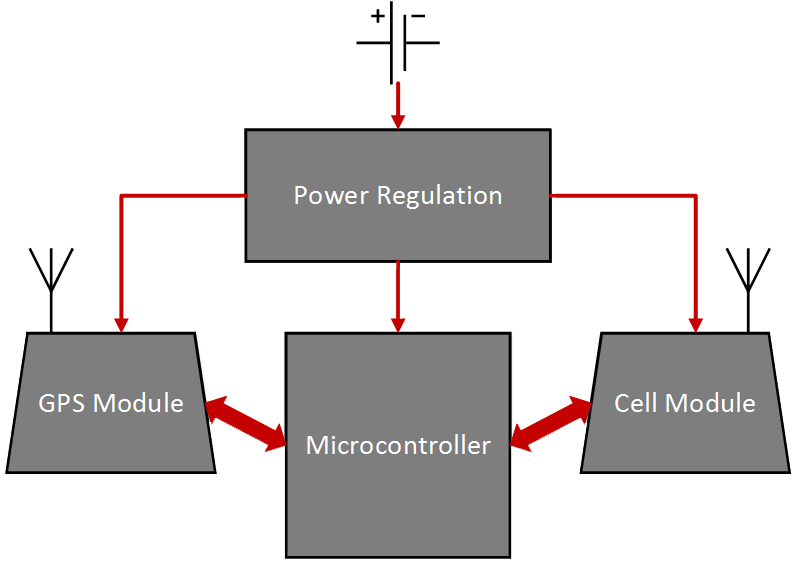
\includegraphics[scale=0.4]{PTD.png}
   \caption{System Diagram}
   \label{fig:sys_diagram}
\end{figure}


\section{Methods}
In this section I will expound upon each of the sub-systems and explain in greater detail their function and components.

The microcontoller that I will use will be the Tiva-C TM4C123G. This microcontroller was chosen because I have worked with it before and I have one 
on hand that can easily be used for prototyping. This microcontroler has plenty of the UART modules that allow for serial communication between the other 
module as well as a hibernation mode that will allow the microcontroller to enter and exit the low-power states required by this project.

The GPS sub-system will consist of three parts.
\begin{itemize}
    \item GPS Module -- Trimble Copernicas 2
    \item GPS Evaluation Board
    \item GPS Antenna -- SPS antenna with SMA Connector
\end{itemize}
The Trible GPS module can update location at a rate of 1Hz and reports it's location via UART transmission. This module was selected because it has great 
reviews and uses the common SMA connector for the antenna. This connector allows for a wide variety of antenna choices.

The cell sub-system chosen for the project also consists of three parts.
\begin{itemize}
    \item Cell Module -- SM5100B
    \item Cell Evaluation Board
    \item Cell Antenna -- Quad-band Duck-bill Antenna
\end{itemize}
The SM5100B module was selected because it can operate on all major US cell carriers. The SIM card of one of these carriers can be seated in the evaluation board 
which connects to the module and antenna. This cell module adds the functionality that the PTD will not change behavior when the SIM card is changed except for the PTD's cell number. The evaluation boards are necessary in 
the case of both the cell and GPS modules to easily interface and prototype the design. The PTD requires two different antennas because GPS and cell signals 
are carried on vary different bands of communication.

The last system that is required is the Power Regulation Circuitry. The circuit needs to source a constant 5 Volts to the microcontroller and 3.3 Volts to 
both of the other modules. This will be done using switching regulators. Switching regulators will be used instead of linear regulators to maintain a low-power 
mode of operation. A linear regulator would provide and source the correct amount of power but would also  drain the battery even when in the low-power state 
of operation.


\section{Resources}
The resources that will be absolutely necessary for this project will be the data sheets of the distinct components. These data sheets will outline the 
function and communication standards that will help me configure and interface correctly with the devices. Other resources will be people that will help 
guide decisions about the design such as Prof. Cripps and Prof. Moon.

The EMI regulations by the FCC can be found in the documents provided in the PTD Specification Document. These documents are also outlined in the References 
Section.

\section{Schedule}
The project is to be completed at the end of November, 2015. This allows me sufficient time to plan and design, prototype, and test the PTD for the next 7 
months. These three phases are outlined in the Gantt Chart in Figure \ref{fig:gantt_schedule}.
\begin{figure}[H]
   \centering
       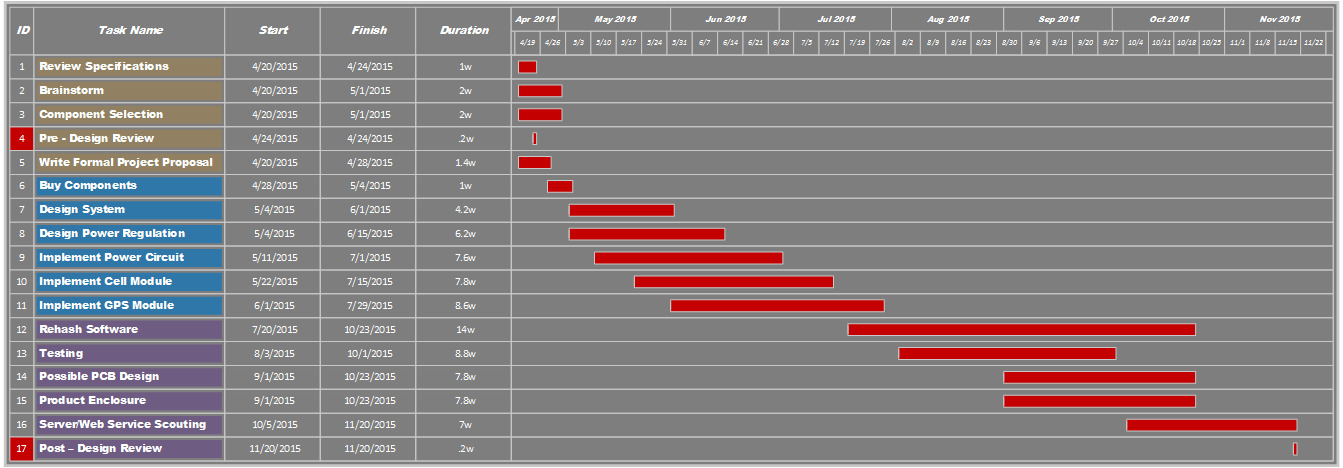
\includegraphics[scale=0.4]{senior_project_gantt.png}
   \caption{Project Schedule}
   \label{fig:gantt_schedule}
\end{figure}

\section{Qualifications}
Another resouce that I have is familiarity with embedded projects. This is due to course work that I completed at Utah State University. The skills 
necessary to design a stable, functional system have been key in completing other projects to date. These projects include:
\begin{itemize}
    \item Custom Computer Case Cooling and Monitoring System
    \item Hardware Keyboard Keylogger
    \item Custom Therostat System
    \item FPGA Butterfly Puf TRNG
\end{itemize}
Each of these projects included unique problems and technical set-backs that have helped me develope problem solving and debugging skills.


\section{Costs}
As can be seen in Figure: \ref{tab:cost}, there are costs associated with the project prototyping that will not be present in the final product.
These costs are a necessary cost in order to easily connect and interface with the discrete modules. The third column shows the cost of the 
component that is attached to an evaluation board and the fourth column shows the cost of the components on their own.

The costs of the cell service will also likely be smaller because such a small amount of data is needed to transmit the device's location. This will 
also depend on the geographical location of interest to the client.
\begin{figure}[H]
   \centering
       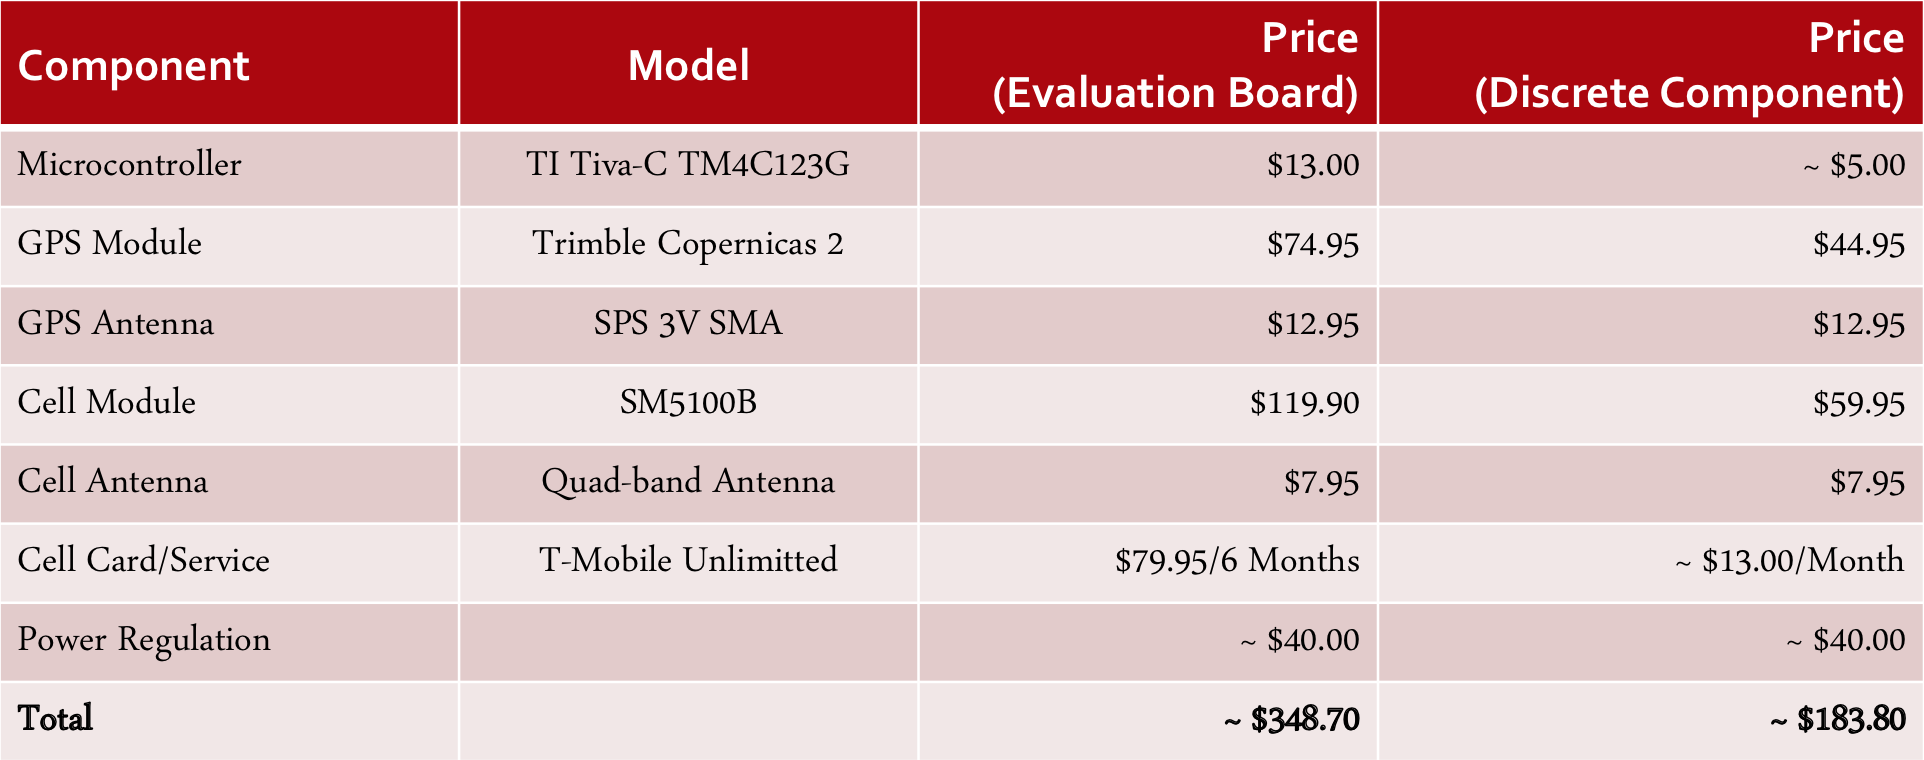
\includegraphics[scale=0.4]{cost_table.png}
   \caption{Project Cost Table}
   \label{tab:cost}
\end{figure}


\section{Conclusion}
The PTD will provide a small low-power passive tracking solution to businesses and enthusients to track their ATVs. The PTD adds another spin on tracking 
devices that currently are not availble on the market because of the unique space and power constraints that ATVs require. Although this project has focused 
on ATVs, the PTD could be installed in any system that has a 12V. batteery such as a truck or snowmobile. 

This product can be expanded past the scope of this project by PCB design as well as enclosure manufacturing. Another future innovation would be to create 
a database hosted on a web server that could be used as a central management hub for clients. This would be of great use to large customers that require 
many PTDs to track their entire fleet. A private inhouse option could also be provide for those businesses that would like to host their own tracking server.

The PTD is unique in the way that it provides the tracking solution. The unique aspects will allow the PTD to be a welcome tracking solution in todays 
economy.


\section{References}
The regulations in the following documents shall be met to allow the PTD to be legally used in most of North America (US and Canada).
\begin{itemize}
    \item The United States (US) FCC Part 15-2008.
    \item Canada's Industry Canada ICES-003:2004 Issue 4.
\end{itemize}

\pagebreak
\section{Appendix A}
\begin{figure}[H]
   \centering
       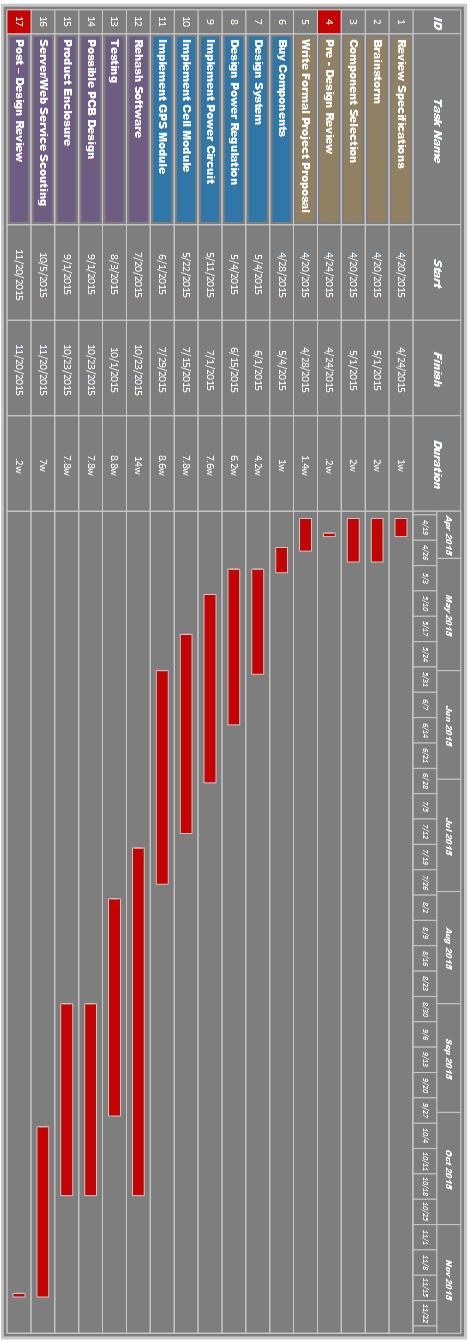
\includegraphics[scale=0.55]{senior_project_gantt_vert.png}
   \caption{Project Schedule Vertical}
   \label{fig:gantt_vertical}
\end{figure}


\end{document}
















